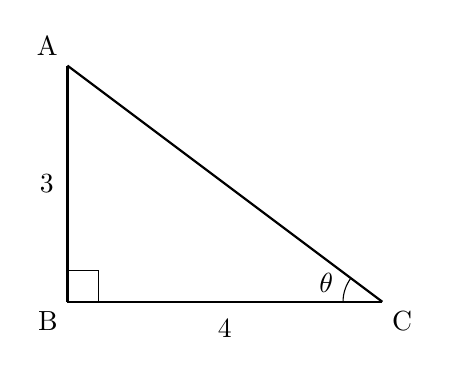
\begin{tikzpicture}

    % Define the coordinates of the triangle vertices
    % B is at origin, A is directly above B, C is to the right of B
    \coordinate (A) at (0, 3);    % Top vertex
    \coordinate (B) at (0, 0);    % Bottom-left vertex (right angle)
    \coordinate (C) at (4, 0);    % Bottom-right vertex
    
    % Draw the triangle sides
    % Side AB (vertical leg)
    \draw[thick] (A) -- (B);
    
    % Side BC (horizontal leg)
    \draw[thick] (B) -- (C);
    
    % Side AC (hypotenuse)
    \draw[thick] (A) -- (C);
    
    % Draw the right angle symbol at vertex B
    % Small square indicating 90 degrees
    \draw (0, 0.4) -- (0.4, 0.4) -- (0.4, 0);
    
    % Draw the angle arc for theta at vertex C
    % Arc showing angle theta
    \draw (3.5, 0) arc (180:143:0.5);
    
    % Label the vertices
    % Point A at top
    \node[above left] at (A) {A};
    
    % Point B at bottom-left
    \node[below left] at (B) {B};
    
    % Point C at bottom-right
    \node[below right] at (C) {C};
    
    % Label the side lengths
    % Side AB has length 3
    \node[left] at (-0.05, 1.5) {3};
    
    % Side BC has length 4
    \node[below] at (2, -0.1) {4};
    
    % Label the angle theta at C
    \node[above left] at (3.5, 0) {$\theta$};
    
    \end{tikzpicture}